\section{Искуственные нейронные сети}

\indent
\indent
Настоящая часть работы предназначена для читателя, не знакомого с 
искуственными нейронными сетями. Здесь будут приведены теоретические 
основы глубокого обучения и рассмотрены сверточные архитектуры, 
используемые в дальнейшей работе.

\subsection{Базовая информация о глубоком обучении}

\indent
\indent
Начнем с рассмотрения одиночного нейрона
 --- перцептрона Розенблатта --- базового элемента, содержащегося в большинстве современных нейросетевых архитектур.
Перцептрон имеет несколько входов и один выход, значение на котором
вычисляется как взвешенная сумма значений входов 
(рисунок \ref{tikzpicture: perceptron}).
Кроме того, обычно
к выходному значению применяется сдвиг и некоторая нелинейная функция, 
называющаяся функцией активации нейрона. Ее предназначение мы обсудим позже.

\begin{figure}[h!]
    \begin{center}
   	    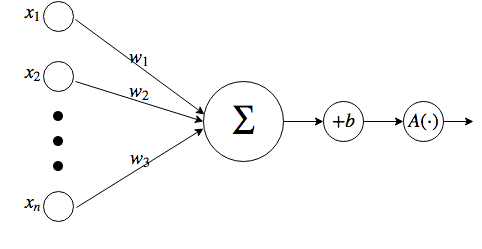
\includegraphics[width=0.6\linewidth]{Perceptron}
   	\end{center}
   	\caption{Схематическое изображение работы одного отдельного нейрона.}
   	\label{tikzpicture: perceptron}
\end{figure}


\indent
\indent
Таким образом, значение на выходе нейрона задается
 выражением \ref{eq:perceptron}.

\begin{equation}\label{eq:perceptron}
    f(\vec{x}) = S(\sum_{i=1}^n x_i w_i + b)
\end{equation}


где $f(\vec{x})$ -- выходное значения нейрона, посчитанное для входов $x_i$,
$w_i$ -- весовые коэффициенты для входов, $b$ -- параметр смещения, 
а $S$ --- нелинейная функция активации.

\indent
\indent
Существуют множество различных функций активации, например, гиперболический
тангенс, логистическая сигмоида или \textit{ReLU}. Перечисленные
функции особенно популярны, так как значения их производных простым образом 
выражаются через значения самой функции (выражение \ref{eq:activations}), 
что, как будет показано далее, позволяет
ускорить процесс обучения нейросети.


\begin{equation}\label{eq:activations}
	\begin{gathered}
	    S(x) = th(x) = \frac{e^x - e^{-x}}{e^x + e^{-x}},    \;   th’(x) = 1 - th(x)^2   \\    
	    S(x) = \sigma(x) = \frac{1}{1 + e^{-x}},   \;   \sigma’(x) = \sigma(x)(1 - \sigma(x)) \\
	    S(x) = ReLU = max(0, x),   \;   ReLU’(x) = \theta(x)
	\end{gathered}
\end{equation}
где $\theta(x)$ -- функция Хэвисайда.


\indent
Одиночный нейрон не способен выразить сложные в наборе
признаков $\vec{x}$, поэтому нейроны объединяют в слои, а их, в свою 
очередь, в многослойные нейросети . Рассмотрим нейронную сеть,
состоящую из нескольких слоев. Пусть количество количество входных признаков
равно $N$, размер скрытого слоя $M$, а выходного -- $P$. Сеть схематично
изображена на рисунке \ref{tikzpicture: fc_net}.
 
 
\begin{figure}[h!]
    \begin{center}
   	    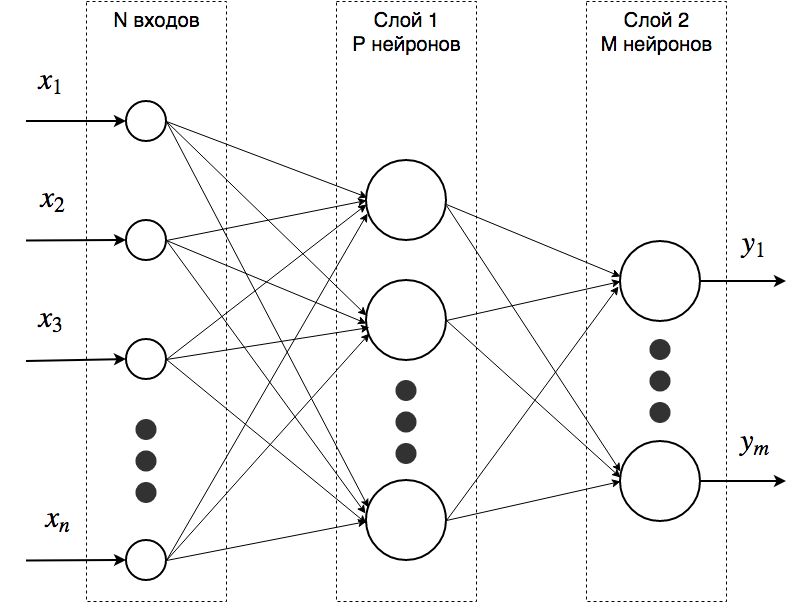
\includegraphics[width=0.9\linewidth]{FC_net}
   	\end{center}
   	\caption{Схематическое изображение полносвязной нейронной сети.}
   	\label{tikzpicture: fc_net}
\end{figure}


 Объединение нейронов в слои.
 Сведение к матрицам
 Вычислительный граф
 Обучение обратным распостранением ошибки.
 
 
\subsection{Сверточные нейронные сети}
Свертка
Пулинг
Сверточная сеть


\subsection{Используемые архитектуры}
В данное работе в качестве базовой неросетевой архитектуры используется
ResNet \cite{resnet}.
